\documentclass[11pt]{article}

% ============================================================================
% PACKAGES
% ============================================================================
\usepackage{amsmath, amssymb, amsthm}
\usepackage{mathtools}      % For \coloneqq and other extensions
\usepackage{algorithm}
\usepackage{algpseudocode}
\usepackage{booktabs}       % For nice tables
\usepackage{array}
\usepackage{graphicx}
\usepackage{xcolor}
\usepackage{hyperref}
\usepackage{enumitem}       % For customized lists
\usepackage{tikz}
\usetikzlibrary{arrows.meta, positioning}

% ============================================================================
% THEOREM ENVIRONMENTS
% ============================================================================
\theoremstyle{plain}
\newtheorem{theorem}{Theorem}[section]
\newtheorem{lemma}[theorem]{Lemma}
\newtheorem{proposition}[theorem]{Proposition}
\newtheorem{corollary}[theorem]{Corollary}

\theoremstyle{definition}
\newtheorem{definition}[theorem]{Definition}
\newtheorem{example}[theorem]{Example}
\newtheorem{remark}[theorem]{Remark}

% ============================================================================
% CUSTOM COMMANDS FOR NOTATION
% ============================================================================
% Bit operations (matching Hamilton's notation)
\newcommand{\XOR}{\mathbin{\veebar}}           % XOR: exclusive or
\newcommand{\AND}{\mathbin{\wedge}}            % AND
\newcommand{\OR}{\mathbin{\vee}}               % OR
\newcommand{\NOT}{\mathord{\sim}}              % NOT (bitwise complement)
\newcommand{\SHL}{\mathbin{\triangleleft}}     % Shift left
\newcommand{\SHR}{\mathbin{\triangleright}}    % Shift right
\newcommand{\ROTL}{\mathbin{\circlearrowleft}} % Rotate left
\newcommand{\ROTR}{\mathbin{\circlearrowright}}% Rotate right

% Convenient shortcuts
\newcommand{\gc}{\mathrm{gc}}                  % Gray code function
\newcommand{\gcinv}{\mathrm{gc}^{-1}}          % Gray code inverse
\newcommand{\bitfn}{\mathrm{bit}}              % bit extraction function
\newcommand{\tsb}{\mathrm{tsb}}                % trailing set bits
\newcommand{\entry}{\mathrm{e}}                % entry point function
\newcommand{\exitpt}{\mathrm{f}}               % exit point function (f for "finish")
\newcommand{\dir}{\mathrm{d}}                  % direction function
\newcommand{\gcr}{\mathrm{gcr}}                % Gray code rank

% Sets
\newcommand{\Z}{\mathbb{Z}}                    % Integers
\newcommand{\N}{\mathbb{N}}                    % Natural numbers
\newcommand{\B}{\mathbb{B}}                    % Binary digits {0,1}

% Other
\newcommand{\encode}{\mathrm{encode}}
\newcommand{\decode}{\mathrm{decode}}

% ============================================================================
% DOCUMENT
% ============================================================================

\title{An Elaborated Proof of Correctness for the\\
Anisotropic Hilbert Curve with Activation Embedding}
\author{Elaboration of \texttt{discrete\_proof.md}}
\date{\today}

\begin{document}
\maketitle

\begin{abstract}
This document provides a detailed, intuitive explanation of how to construct
a Hilbert curve on a \emph{dyadic box}---an $n$-dimensional rectangular grid
where each axis has length $2^{m_j}$ for possibly different values of $m_j$.
The key innovation is the \textbf{activation embedding} technique, which
correctly handles the transition when new axes ``activate'' as the algorithm
descends through bit-planes. We prove that the resulting \texttt{encode} and
\texttt{decode} functions are exact inverses, and that the curve visits
adjacent lattice points at each step (lattice continuity). This document
elaborates on the concise proof in \texttt{discrete\_proof.md}, adding
intuitive explanations, careful variable definitions, and worked examples.
\end{abstract}

\tableofcontents
\newpage

% ============================================================================
\section{Introduction and Motivation}
% ============================================================================

\subsection{What is a Hilbert Curve?}

A \textbf{Hilbert curve} is a way to visit every point in a grid exactly once,
taking only unit steps (moving to an adjacent cell). In 2D, you've probably
seen the familiar ``U-shaped'' recursive pattern:

\begin{center}
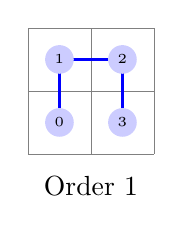
\begin{tikzpicture}[scale=0.8]
    % Order 1 Hilbert curve (2x2)
    \draw[step=1, gray, very thin] (0,0) grid (2,2);
    \draw[thick, blue, ->] (0.5,0.5) -- (0.5,1.5) -- (1.5,1.5) -- (1.5,0.5);
    \foreach \x/\y/\n in {0.5/0.5/0, 0.5/1.5/1, 1.5/1.5/2, 1.5/0.5/3} {
        \node at (\x,\y) [circle, fill=blue!20, inner sep=2pt] {\tiny \n};
    }
    \node at (1, -0.5) {Order 1};
\end{tikzpicture}
\hspace{2cm}
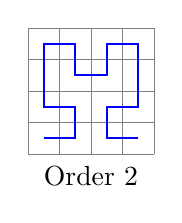
\begin{tikzpicture}[scale=0.4]
    % Order 2 Hilbert curve (4x4) - simplified representation
    \draw[step=1, gray, very thin] (0,0) grid (4,4);
    \draw[thick, blue]
        (0.5,0.5) -- (1.5,0.5) -- (1.5,1.5) -- (0.5,1.5) --
        (0.5,2.5) -- (0.5,3.5) -- (1.5,3.5) -- (1.5,2.5) --
        (2.5,2.5) -- (2.5,3.5) -- (3.5,3.5) -- (3.5,2.5) --
        (3.5,1.5) -- (2.5,1.5) -- (2.5,0.5) -- (3.5,0.5);
    \node at (2, -0.7) {Order 2};
\end{tikzpicture}
\end{center}

The key property is \textbf{locality}: points that are close along the curve
tend to be close in the grid. This makes Hilbert curves useful for databases,
image processing, and scientific computing.

\subsection{The Problem: Unequal Side Lengths}

Hamilton's classic algorithms work on \textbf{hypercubes}---grids where every
axis has the same length $2^m$. But what if we want a $4 \times 8$ grid, or
more generally, a grid where axis $j$ has length $2^{m_j}$ for different values
of $m_j$?

\begin{example}[A $4 \times 2$ Grid]
Consider $n = 2$ dimensions with $m_0 = 2$ (so the $x$-axis has $2^2 = 4$ points)
and $m_1 = 1$ (so the $y$-axis has $2^1 = 2$ points). We want to visit all
$4 \times 2 = 8$ points exactly once, taking unit steps:

\begin{center}
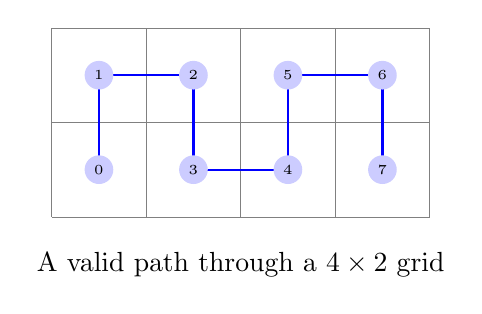
\begin{tikzpicture}[scale=1.2]
    \draw[step=1, gray, very thin] (0,0) grid (4,2);
    % A valid Hilbert-like path
    \draw[thick, blue, ->]
        (0.5,0.5) -- (0.5,1.5) -- (1.5,1.5) -- (1.5,0.5) --
        (2.5,0.5) -- (2.5,1.5) -- (3.5,1.5) -- (3.5,0.5);
    \foreach \x/\y/\n in {0.5/0.5/0, 0.5/1.5/1, 1.5/1.5/2, 1.5/0.5/3,
                          2.5/0.5/4, 2.5/1.5/5, 3.5/1.5/6, 3.5/0.5/7} {
        \node at (\x,\y) [circle, fill=blue!20, inner sep=2pt] {\tiny \n};
    }
    \node at (2, -0.5) {A valid path through a $4 \times 2$ grid};
\end{tikzpicture}
\end{center}
\end{example}

This is the \textbf{anisotropic} (unequal-dimension) Hilbert curve problem.

\subsection{Hamilton's Approach and the Bug}

Hamilton's 2008 paper introduced ``compact Hilbert indices'' to handle unequal
dimensions. The idea is elegant: at each recursion level, some axes are
``active'' (still have bits to contribute) while others are ``inactive''
(already exhausted their precision). However, \textbf{Hamilton's original
algorithm has a subtle bug} in how it handles the transition when axes
activate.

The levels for a 4x4 start at level 2 for the coarsest, then level 1 for refinement.
At each level there are k=2 axes active. For a 4x2, the coarsest level,
level 2, has k=1 axis active. Then at level 1 it has k=2 axes active.

The bug manifests as follows: when moving from a level with $k$ active axes
to a level with $k' > k$ active axes, the ``direction'' parameter $d$ must be
\textbf{reinterpreted}. Hamilton treats $d$ as a \emph{positional index}
(``the $d$-th axis in the current list''), but at activation boundaries, it
must be treated as a \emph{physical axis label} (``axis number $j$ in the
original coordinate system'').

\textbf{The fix} is called \textbf{activation embedding}: when new axes
activate, we embed the state $(e, d)$ from the smaller active set into the
larger one by:
\begin{enumerate}
    \item Copying bits of $e$ to their corresponding physical axes
    \item Setting newly activated axes' bits to 0
    \item \textbf{Re-indexing $d$} to point to the same physical axis in the
          new, larger axis list
\end{enumerate}

This document proves that with this fix, the algorithm is correct.

\subsection{What We Will Prove}

\begin{enumerate}
    \item \textbf{Bijection}: The \texttt{encode} and \texttt{decode} functions
          are exact inverses. Every point maps to a unique index, and vice versa.
    \item \textbf{Lattice Continuity}: Consecutive indices correspond to
          adjacent lattice points: $|H_m(h+1) - H_m(h)|_1 = 1$ for all valid $h$.
\end{enumerate}

% ============================================================================
\section{Notation and Definitions}
% ============================================================================

Before diving into the proof, let's carefully define all the notation.
This section is your reference for ``what does this symbol mean?''

\subsection{Basic Setup}

\begin{definition}[Dimension and Precision]
We work in $n$ dimensions, indexed $j = 0, 1, \ldots, n-1$.

Each axis $j$ has \textbf{precision} $m_j \in \N$ (a non-negative integer),
meaning axis $j$ has $2^{m_j}$ discrete points, numbered $0, 1, \ldots, 2^{m_j} - 1$.

We write $\mathbf{m} = (m_0, m_1, \ldots, m_{n-1})$ for the vector of precisions.
\end{definition}

\begin{definition}[The Dyadic Box $P(\mathbf{m})$]
The \textbf{dyadic box} is the set of all lattice points:
\[
P(\mathbf{m}) = \{0, 1, \ldots, 2^{m_0}-1\} \times \{0, 1, \ldots, 2^{m_1}-1\}
               \times \cdots \times \{0, 1, \ldots, 2^{m_{n-1}}-1\}
\]
(The term dyadic box is used in harmonic analysis and measure theory.)
A point $\mathbf{p} \in P(\mathbf{m})$ is an $n$-tuple $\mathbf{p} = (p_0, p_1, \ldots, p_{n-1})$
where $0 \le p_j < 2^{m_j}$.
\end{definition}

\begin{definition}[Total Bits $M$]
The total number of bits needed to specify a point is:
\[
M = \sum_{j=0}^{n-1} m_j
\]
The number of points in the box is $|P(\mathbf{m})| = 2^M$.
\end{definition}

\begin{example}
For a $4 \times 2$ grid: $n = 2$, $m_0 = 2$, $m_1 = 1$, so $M = 2 + 1 = 3$
and there are $2^3 = 8$ points.
\end{example}

\subsection{Bit Operations}

\begin{definition}[Bit Extraction]
For a non-negative integer $a$ and bit position $k \ge 0$:
\[
\bitfn(a, k) = \left\lfloor \frac{a}{2^k} \right\rfloor \mod 2 =
\begin{cases}
1 & \text{if the $k$-th bit of $a$ is set} \\
0 & \text{otherwise}
\end{cases}
\]
Bit 0 is the \textbf{least significant bit} (rightmost).
\end{definition}

\begin{example}
For $a = 13 = [1101]_2$ (binary):
\begin{itemize}
    \item $\bitfn(13, 0) = 1$ (the rightmost bit)
    \item $\bitfn(13, 1) = 0$
    \item $\bitfn(13, 2) = 1$
    \item $\bitfn(13, 3) = 1$ (the leftmost bit)
\end{itemize}
\end{example}

\begin{definition}[Bitwise XOR]
The \textbf{exclusive-or} operation $a \XOR b$ flips each bit where $a$ and $b$
differ:
\[
\bitfn(a \XOR b, k) = \bitfn(a, k) + \bitfn(b, k) \mod 2
\]
\end{definition}

\begin{example}
$13 \XOR 6 = [1101]_2 \XOR [0110]_2 = [1011]_2 = 11$.
\end{example}

\begin{definition}[Bit Rotation]
For an $n$-bit value $b$ and rotation amount $r$:
\begin{itemize}
    \item \textbf{Right rotation}: $b \ROTR r$ shifts bits right by $r$ positions,
          wrapping around. Bit $k$ of $b$ becomes bit $(k - r) \mod n$ of the result.
    \item \textbf{Left rotation}: $b \ROTL r$ shifts bits left by $r$ positions,
          wrapping around. Bit $k$ of $b$ becomes bit $(k + r) \mod n$ of the result.
\end{itemize}
These are inverses: $(b \ROTR r) \ROTL r = b$.
\end{definition}

\begin{example}
With $n = 4$ bits, let $b = [1011]_2 = 11$:
\begin{itemize}
    \item $b \ROTR 1 = [1101]_2 = 13$ (rightmost bit wraps to leftmost)
    \item $b \ROTL 1 = [0111]_2 = 7$ (leftmost bit wraps to rightmost)
\end{itemize}
\end{example}

\subsection{Gray Code}

The Gray code is fundamental to Hilbert curves because it provides a way to
enumerate hypercube corners such that consecutive corners differ in exactly
one coordinate.

\begin{definition}[Binary Reflected Gray Code]
The \textbf{Gray code} function $\gc: \{0, \ldots, 2^n - 1\} \to \{0, \ldots, 2^n - 1\}$
is defined by:
\[
\gc(i) = i \XOR (i \SHR 1)
\]
where $i \SHR 1$ means ``shift $i$ right by 1 bit'' (i.e., $\lfloor i/2 \rfloor$).
\end{definition}

\begin{example}[3-bit Gray Code]
\begin{center}
\begin{tabular}{c|c|c|c}
$i$ & Binary of $i$ & $\gc(i)$ & Binary of $\gc(i)$ \\
\midrule
0 & 000 & 0 & 000 \\
1 & 001 & 1 & 001 \\
2 & 010 & 3 & 011 \\
3 & 011 & 2 & 010 \\
4 & 100 & 6 & 110 \\
5 & 101 & 7 & 111 \\
6 & 110 & 5 & 101 \\
7 & 111 & 4 & 100 \\
\end{tabular}
\end{center}
Notice: consecutive rows of $\gc(i)$ differ in exactly one bit!
\end{example}

\begin{definition}[Gray Code Inverse]
The inverse $\gcinv$ recovers $i$ from $\gc(i)$. It satisfies:
\[
\bitfn(i, k) = \sum_{j=k}^{n-1} \bitfn(\gc(i), j) \mod 2
\]
In other words, bit $k$ of $i$ is the XOR of all bits of $\gc(i)$ from position
$k$ to the most significant bit.
\end{definition}

\begin{definition}[Dimension of Change $\mathrm{g}(i)$]
When moving from $\gc(i)$ to $\gc(i+1)$, exactly one bit changes. We define:
\[
\mathrm{g}(i) = k \quad \text{where} \quad \gc(i) \XOR \gc(i+1) = 2^k
\]
Hamilton proves that $\mathrm{g}(i) = \tsb(i)$, the number of \textbf{trailing
set bits} in the binary representation of $i$.
\end{definition}

\begin{example}
\begin{itemize}
    \item $i = 0 = [000]_2$: zero trailing 1s, so $\mathrm{g}(0) = 0$
    \item $i = 1 = [001]_2$: one trailing 1, so $\mathrm{g}(1) = 1$
    \item $i = 3 = [011]_2$: two trailing 1s, so $\mathrm{g}(3) = 2$
    \item $i = 5 = [101]_2$: one trailing 1, so $\mathrm{g}(5) = 1$
\end{itemize}
\end{example}

\subsection{Hamilton's Entry/Exit/Direction Functions}

These functions describe how sub-hypercubes connect in the Hilbert curve.
These are the sub-hypercubes that are the children at the current order.

\begin{definition}[Entry Point $\entry(i)$]
The \textbf{entry point} $\entry(i)$ is the corner of the $i$-th sub-hypercube
where the Hilbert curve enters. Hamilton proves:
\[
\entry(i) = \begin{cases}
0 & \text{if } i = 0 \\
\gc\left(2 \left\lfloor \frac{i-1}{2} \right\rfloor\right) & \text{if } i > 0
\end{cases}
\]
\end{definition}
If you're at level $s$ processing some region, that region has $2^{k_s}$ children,
one for each combination of low are high along each active axis.

\begin{definition}[Exit Point $\exitpt(i)$]
The \textbf{exit point} $\exitpt(i)$ is where the curve leaves sub-hypercube $i$.
It relates to the entry point by:
\[
\exitpt(i) = \entry(i) \XOR 2^{\dir(i)}
\]
meaning entry and exit differ in exactly one bit (they're adjacent corners).
\end{definition}

\begin{definition}[Intra-subcube Direction $\dir(i)$]
The \textbf{direction} $\dir(i) \in \Z_n$ tells which axis connects $\entry(i)$
to $\exitpt(i)$. Hamilton proves:
\[
\dir(i) = \begin{cases}
0 & \text{if } i = 0 \\
\mathrm{g}(i-1) \mod n & \text{if } i > 0 \text{ and } i \text{ is even} \\
\mathrm{g}(i) \mod n & \text{if } i \text{ is odd}
\end{cases}
\]
\end{definition}

\begin{definition}[Inter-subcube Direction $\mathrm{g}(i)$]
This is the axis along which sub-hypercube $i$ connects to sub-hypercube $i+1$.
As noted above, $\mathrm{g}(i) = \tsb(i)$.
\end{definition}

The crucial relationship linking consecutive sub-hypercubes is:
\begin{equation}
\entry(i+1) = \entry(i) \XOR 2^{\dir(i)} \XOR 2^{\mathrm{g}(i)}
\label{eq:entry-recursion}
\end{equation}

\textbf{Intuition}: The exit of sub-hypercube $i$ is $\exitpt(i) = \entry(i) \XOR 2^{\dir(i)}$.
Sub-hypercubes $i$ and $i+1$ are adjacent along axis $\mathrm{g}(i)$, so their
connecting corners differ by $2^{\mathrm{g}(i)}$. Hence
$\entry(i+1) = \exitpt(i) \XOR 2^{\mathrm{g}(i)} = \entry(i) \XOR 2^{\dir(i)} \XOR 2^{\mathrm{g}(i)}$.

\subsubsection{Diagram: One Level of Recursion in 2D}

The following diagram shows how a single level of recursion works in 2D.
We have a parent square divided into 4 children. The index $i \in \{0,1,2,3\}$
indicates the \textbf{visit order} (not the spatial position). The Gray code
$\gc(i)$ gives the corner label (spatial position) of each child.

\begin{center}
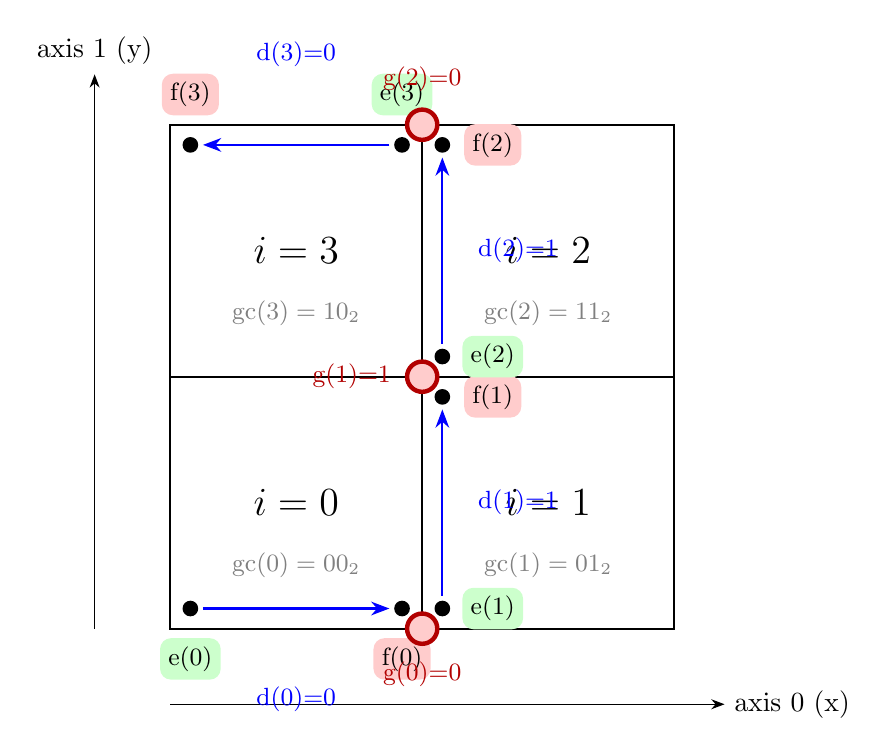
\begin{tikzpicture}[scale=3.2, >=Stealth,
    every node/.style={font=\normalsize},
    corner/.style={circle, fill=black, inner sep=2pt},
    elabel/.style={fill=green!20, rounded corners, inner sep=3pt, font=\small},
    flabel/.style={fill=red!20, rounded corners, inner sep=3pt, font=\small}]

    % Draw the 4 quadrants
    \draw[thick] (0,0) rectangle (2,2);
    \draw[thick] (1,0) -- (1,2);
    \draw[thick] (0,1) -- (1,1) (1,1) -- (2,1);

    % Label axes
    \draw[->] (-0.3, 0) -- (-0.3, 2.2) node[above] {axis 1 (y)};
    \draw[->] (0, -0.3) -- (2.2, -0.3) node[right] {axis 0 (x)};

    % Quadrant labels: visit order i and gray code gc(i)
    % gc(0)=0=[00], gc(1)=1=[01], gc(2)=3=[11], gc(3)=2=[10]
    % So: i=0 at [00]=bottom-left, i=1 at [01]=bottom-right,
    %     i=2 at [11]=top-right, i=3 at [10]=top-left

    % Child i=0: gc(0)=0=[00] -> bottom-left quadrant
    \node at (0.5, 0.5) [font=\Large\bfseries] {$i=0$};
    \node at (0.5, 0.25) [font=\small, gray] {$\gc(0)=00_2$};

    % Child i=1: gc(1)=1=[01] -> bottom-right quadrant
    \node at (1.5, 0.5) [font=\Large\bfseries] {$i=1$};
    \node at (1.5, 0.25) [font=\small, gray] {$\gc(1)=01_2$};

    % Child i=2: gc(2)=3=[11] -> top-right quadrant
    \node at (1.5, 1.5) [font=\Large\bfseries] {$i=2$};
    \node at (1.5, 1.25) [font=\small, gray] {$\gc(2)=11_2$};

    % Child i=3: gc(3)=2=[10] -> top-left quadrant
    \node at (0.5, 1.5) [font=\Large\bfseries] {$i=3$};
    \node at (0.5, 1.25) [font=\small, gray] {$\gc(3)=10_2$};

    % CORRECTED entry/exit positions and arrows based on:
    % i=0: e(0)=00 local -> (0,0) global, f(0)=01 local -> (1,0) global, d(0)=0 (horizontal)
    % i=1: e(1)=00 local -> (1,0) global, f(1)=10 local -> (1,1) global, d(1)=1 (vertical)
    % i=2: e(2)=00 local -> (1,1) global, f(2)=10 local -> (1,2) global, d(2)=1 (vertical)
    % i=3: e(3)=11 local -> (1,2) global, f(3)=10 local -> (0,2) global, d(3)=0 (horizontal)
    % Global path: (0,0) -> (1,0) -> (1,1) -> (1,2) -> (0,2)

    % Draw entry/exit for child i=0 (bottom-left quadrant)
    % Entry at (0,0), Exit at (1,0), arrow horizontal (d=0 means axis 0 = x)
    \node[corner] at (0.08, 0.08) {};
    \node[elabel] at (0.08, -0.12) {$\entry(0)$};
    \node[corner] at (0.92, 0.08) {};
    \node[flabel] at (0.92, -0.12) {$\exitpt(0)$};
    \draw[->, thick, blue] (0.13, 0.08) -- (0.87, 0.08);
    \node[blue, font=\small] at (0.5, -0.28) {$\dir(0){=}0$};

    % Draw entry/exit for child i=1 (bottom-right quadrant)
    % Entry at (1,0), Exit at (1,1), arrow vertical (d=1 means axis 1 = y)
    \node[corner] at (1.08, 0.08) {};
    \node[elabel] at (1.28, 0.08) {$\entry(1)$};
    \node[corner] at (1.08, 0.92) {};
    \node[flabel] at (1.28, 0.92) {$\exitpt(1)$};
    \draw[->, thick, blue] (1.08, 0.13) -- (1.08, 0.87);
    \node[blue, font=\small] at (1.38, 0.5) {$\dir(1){=}1$};

    % Draw entry/exit for child i=2 (top-right quadrant)
    % Entry at (1,1), Exit at (1,2), arrow vertical (d=1 means axis 1 = y)
    \node[corner] at (1.08, 1.08) {};
    \node[elabel] at (1.28, 1.08) {$\entry(2)$};
    \node[corner] at (1.08, 1.92) {};
    \node[flabel] at (1.28, 1.92) {$\exitpt(2)$};
    \draw[->, thick, blue] (1.08, 1.13) -- (1.08, 1.87);
    \node[blue, font=\small] at (1.38, 1.5) {$\dir(2){=}1$};

    % Draw entry/exit for child i=3 (top-left quadrant)
    % Entry at (1,2), Exit at (0,2), arrow horizontal going left (d=0 means axis 0 = x)
    \node[corner] at (0.92, 1.92) {};
    \node[elabel] at (0.92, 2.12) {$\entry(3)$};
    \node[corner] at (0.08, 1.92) {};
    \node[flabel] at (0.08, 2.12) {$\exitpt(3)$};
    \draw[->, thick, blue] (0.87, 1.92) -- (0.13, 1.92);
    \node[blue, font=\small] at (0.5, 2.28) {$\dir(3){=}0$};

    % Draw the inter-subcube connections (g(i) directions)
    % These connect f(i) to e(i+1), which are the SAME GLOBAL POINT
    % The dashed arrows show conceptual adjacency along axis g(i)

    % g(0)=0: f(0)=(1,0) connects to e(1)=(1,0) - same point, along axis 0
    % Show this as a small marker at the shared corner
    \draw[ultra thick, red!70!black, fill=red!20] (1, 0) circle (0.06);
    \node[red!70!black, font=\small] at (1.0, -0.18) {$\mathrm{g}(0){=}0$};

    % g(1)=1: f(1)=(1,1) connects to e(2)=(1,1) - same point, along axis 1
    \draw[ultra thick, red!70!black, fill=red!20] (1, 1) circle (0.06);
    \node[red!70!black, font=\small] at (0.72, 1.0) {$\mathrm{g}(1){=}1$};

    % g(2)=0: f(2)=(1,2) connects to e(3)=(1,2) - same point, along axis 0
    \draw[ultra thick, red!70!black, fill=red!20] (1, 2) circle (0.06);
    \node[red!70!black, font=\small] at (1.0, 2.18) {$\mathrm{g}(2){=}0$};

\end{tikzpicture}
\end{center}

\textbf{Reading the diagram:}
\begin{itemize}
    \item The large numbers ($i=0,1,2,3$) show \textbf{visit order}.
    \item The gray labels $\gc(i)$ show the \textbf{corner label} (spatial position):
          which quadrant in binary coordinates $[\text{bit}_1, \text{bit}_0]$.
    \item \textcolor{green!50!black}{Green} = entry point $\entry(i)$;
          \textcolor{red!70!black}{Pink background} = exit point $\exitpt(i)$.
    \item \textcolor{blue}{Blue arrows} show $\dir(i)$: the axis connecting entry to exit
          within each child. When $\dir(i)=0$, the arrow is horizontal (along axis 0);
          when $\dir(i)=1$, the arrow is vertical (along axis 1).
    \item \textcolor{red!70!black}{Red circles} mark the shared corners where
          $\exitpt(i) = \entry(i+1)$ in \emph{global} coordinates. The label
          $\mathrm{g}(i)$ indicates the axis along which the adjacent quadrants meet.
\end{itemize}

\textbf{Key observations:}
\begin{enumerate}
    \item The visit order follows the Gray code: $\gc(0)=00$, $\gc(1)=01$,
          $\gc(2)=11$, $\gc(3)=10$. Consecutive children differ in one bit
          (are spatially adjacent along axis $\mathrm{g}(i)$).
    \item In \emph{global} coordinates, $\exitpt(i) = \entry(i+1)$---the curve is continuous!
          The \emph{local} corner labels differ by $2^{\mathrm{g}(i)}$, but when mapped
          to global positions, they coincide at the shared face between adjacent quadrants.
    \item The entry/exit corners are where the curve enters/leaves each child.
          The full path \emph{within} each child will be determined by
          recursing to the next level.
    \item The global path through the corners is:
          $(0,0) \to (1,0) \to (1,1) \to (1,2) \to (0,2)$.
\end{enumerate}

\begin{center}
\begin{tabular}{c|cccc|c}
\toprule
$i$ & $\gc(i)$ & $\entry(i)$ & $\exitpt(i)$ & $\dir(i)$ & $\mathrm{g}(i)$ \\
\midrule
0 & $00_2$ & $00_2$ & $01_2$ & 0 & 0 \\
1 & $01_2$ & $00_2$ & $10_2$ & 1 & 1 \\
2 & $11_2$ & $00_2$ & $10_2$ & 1 & 0 \\
3 & $10_2$ & $11_2$ & $10_2$ & 0 & --- \\
\bottomrule
\end{tabular}
\end{center}

Note: $\entry(i)$ and $\exitpt(i)$ are corner labels \emph{within} each child's
local coordinate system (the child's own $2\times 2$ grid of corners), not
global coordinates. For example, $\entry(3)=11_2$ means ``top-right corner of
child 3's local frame,'' which happens to be at a specific global position.

\subsection{The $T$-Transform}

The $T$-transform is the core operation that ``reorients'' the coordinate system
as we descend into sub-hypercubes.

\begin{definition}[The $T$-Transform]
For an $n$-bit entry mask $e$ and direction $d \in \Z_n$, define:
\[
T_{(e,d)}(b) = (b \XOR e) \ROTR (d + 1)
\]
This is a bijection (composition of two bijections: XOR and rotation).
\end{definition}

\textbf{What does $T$ do geometrically?}
\begin{itemize}
    \item The XOR by $e$ \textbf{reflects} the hypercube: axes where $\bitfn(e, j) = 1$
          get flipped (0 becomes 1 and vice versa).
    \item The rotation by $d+1$ \textbf{permutes the axes}: what was axis $j$
          becomes axis $(j - d - 1) \mod n$.
\end{itemize}

The key property is that $T$ \textbf{preserves adjacency}: if two corners differ
in one bit, their transforms also differ in one bit (just a different bit position
after rotation).

\begin{definition}[Inverse $T$-Transform]
Hamilton shows:
\[
T_{(e,d)}^{-1}(b) = (b \ROTL (d+1)) \XOR e
\]
or equivalently: $T_{(e,d)}^{-1} = T_{(e \ROTR (d+1), n-d-1)}$.
\end{definition}

\begin{example}[{$T$-Transform with $n=3$, $e=5=[101]_2$, $d=1$}]
Let $b = 3 = [011]_2$.
\begin{enumerate}
    \item XOR with $e$: $b \XOR e = [011]_2 \XOR [101]_2 = [110]_2 = 6$
    \item Rotate right by $d+1 = 2$: $[110]_2 \ROTR 2 = [101]_2 = 5$
\end{enumerate}
So $T_{(5,1)}(3) = 5$.
\end{example}

\subsection{The State Update Rule}

When processing a sub-hypercube with index $w$ in the Gray code ordering,
Hamilton's state update rule transforms $(e, d)$ for the next level:

\begin{align}
e &\leftarrow e \XOR \left( \entry(w) \ROTL (d+1) \right) \label{eq:state-e} \\
d &\leftarrow (d + \dir(w) + 1) \mod n \label{eq:state-d}
\end{align}

\textbf{Intuition}: We're composing transforms. After entering sub-hypercube $w$,
the ``local'' orientation inside that sub-hypercube has its own entry point
$\entry(w)$ and direction $\dir(w)$. These get composed with the current
global transform to give the new global transform.

% ============================================================================
\section{The Anisotropic Setting: Activation}
% ============================================================================

Now we extend to unequal dimensions. The key concept is \textbf{activation}:
at each level, only some axes are ``active'' (still have bits to process).

\subsection{Levels Instead of Bit-Planes}

\begin{definition}[Level $s$]
We use \textbf{level} $s \in \{1, 2, \ldots, m_{\max}\}$ where $m_{\max} = \max_j m_j$.

Level $s$ corresponds to bit-plane $i = s - 1$ in Hamilton's notation. We process
levels from $s = m_{\max}$ down to $s = 1$.

\textbf{Axis $j$ is active at level $s$} if and only if $m_j \ge s$.
\end{definition}

\textbf{Why this convention?} At level $s$, we're extracting the $(s-1)$-th bit
from each active axis. An axis with precision $m_j$ has bits $0, 1, \ldots, m_j - 1$,
so it's active at levels $1, 2, \ldots, m_j$, i.e., when $s \le m_j$.

\begin{example}[$4 \times 8$ Grid]
Let $n = 2$, $m_0 = 2$, $m_1 = 3$, so $m_{\max} = 3$.
\begin{itemize}
    \item Level 3: Axis 0 active? $m_0 = 2 \ge 3$? No. Axis 1 active? $m_1 = 3 \ge 3$? Yes.
          \textbf{Only axis 1 is active.}
    \item Level 2: Axis 0 active? $m_0 = 2 \ge 2$? Yes. Axis 1 active? Yes.
          \textbf{Both axes active.}
    \item Level 1: Both axes active ($m_0 = 2 \ge 1$, $m_1 = 3 \ge 1$).
\end{itemize}
\end{example}

\subsection{Ordered Active Axis Lists}

\begin{definition}[Priority Order $\prec_\pi$]
We fix a total order on axes by:
\[
j \prec_\pi j' \iff (m_j, j) < (m_{j'}, j') \text{ lexicographically}
\]
This means: \textbf{shorter dimensions come first}; ties broken by axis index.
\end{definition}

\begin{example}
For $m_0 = 2$, $m_1 = 3$, $m_2 = 2$:
\begin{itemize}
    \item Compare axes 0 and 1: $(m_0, 0) = (2, 0)$ vs $(m_1, 1) = (3, 1)$.
          Since $2 < 3$, we have $0 \prec_\pi 1$.
    \item Compare axes 0 and 2: $(2, 0)$ vs $(2, 2)$. Same $m$, but $0 < 2$,
          so $0 \prec_\pi 2$.
    \item Compare axes 1 and 2: $(3, 1)$ vs $(2, 2)$. Since $2 < 3$, we have
          $2 \prec_\pi 1$.
\end{itemize}
Full order: $0 \prec_\pi 2 \prec_\pi 1$.
\end{example}

\begin{definition}[Active Axis List $A_s$]
At level $s$, the \textbf{active axis list} is:
\[
A_s = [a^{(s)}_0, a^{(s)}_1, \ldots, a^{(s)}_{k_s - 1}]
\]
where $\{a^{(s)}_t\} = \{j : m_j \ge s\}$ listed in increasing $\prec_\pi$ order,
and $k_s = |A_s|$ is the number of active axes.
\end{definition}

\textbf{Key Property}: $A_{s+1} \subseteq A_s$ (as $s$ decreases, more axes activate).

\begin{example}[Continuing the $4 \times 8$ Example]
With $m_0 = 2$, $m_1 = 3$:
\begin{itemize}
    \item Level 3: Active set is $\{1\}$ (only $m_1 \ge 3$). So $A_3 = [1]$, $k_3 = 1$.
    \item Level 2: Active set is $\{0, 1\}$. Priority order: $0 \prec_\pi 1$
          (since $m_0 = 2 < m_1 = 3$). So $A_2 = [0, 1]$, $k_2 = 2$.
    \item Level 1: Same as level 2. $A_1 = [0, 1]$, $k_1 = 2$.
\end{itemize}
\end{example}

\subsection{Packing Bits into Level Words}

At each level, we extract one bit from each active axis and pack them into
a single integer.

\begin{definition}[Level Bit-Plane Word $\ell_s(p)$]
For a point $\mathbf{p} \in P(\mathbf{m})$, define the $k_s$-bit integer:
\[
\ell_s(\mathbf{p}) = \sum_{t=0}^{k_s - 1} \bitfn(p_{a^{(s)}_t}, s-1) \cdot 2^t
\]
\end{definition}

\textbf{What this means}: $\ell_s(\mathbf{p})$ has one bit from each active axis.
Bit $t$ of $\ell_s(\mathbf{p})$ is the $(s-1)$-th bit of coordinate $p_{a^{(s)}_t}$
(the $t$-th active axis at level $s$).

\begin{example}
Continuing with $m_0 = 2$, $m_1 = 3$. Let $\mathbf{p} = (2, 5) = ([10]_2, [101]_2)$.
\begin{itemize}
    \item Level 3: $A_3 = [1]$, $k_3 = 1$. Extract bit $3-1=2$ from $p_1 = 5 = [101]_2$.
          $\bitfn(5, 2) = 1$. So $\ell_3(\mathbf{p}) = 1$.
    \item Level 2: $A_2 = [0, 1]$, $k_2 = 2$. Extract bit 1 from each:
          $\bitfn(p_0, 1) = \bitfn(2, 1) = 1$ and $\bitfn(p_1, 1) = \bitfn(5, 1) = 0$.
          So $\ell_2(\mathbf{p}) = 1 \cdot 2^0 + 0 \cdot 2^1 = 1$.
    \item Level 1: Extract bit 0: $\bitfn(2, 0) = 0$, $\bitfn(5, 0) = 1$.
          So $\ell_1(\mathbf{p}) = 0 \cdot 2^0 + 1 \cdot 2^1 = 2$.
\end{itemize}
\end{example}

% ============================================================================
\section{The Encode and Decode Algorithms}
% ============================================================================

\subsection{Variable-Width Index Representation}

The Hilbert index $h$ is built from \textbf{variable-width digits}. At each
level $s$, we produce a $k_s$-bit ``digit'' $w_s$.

\begin{definition}[Index Representation]
The index $h$ is represented as:
\[
h = (w_{m_{\max}} \,|\, w_{m_{\max}-1} \,|\, \cdots \,|\, w_1)
\]
where $w_s \in \{0, \ldots, 2^{k_s} - 1\}$ is a $k_s$-bit digit.

The total bit-length is $\sum_{s=1}^{m_{\max}} k_s = \sum_{j=0}^{n-1} m_j = M$.
\end{definition}

\textbf{How to convert to/from an integer}: The digits are concatenated with
most-significant first. If we write $h$ in binary, the first $k_{m_{\max}}$
bits are $w_{m_{\max}}$, the next $k_{m_{\max}-1}$ bits are $w_{m_{\max}-1}$,
and so on.

\subsection{The Per-Level Transform $\Phi$}

At each level, we convert between the level word $\ell_s$ (which describes
the point's position) and the index digit $w_s$ (which goes into the Hilbert index).

\begin{definition}[Per-Level Bijection $\Phi$]
For dimension $k$, entry $e$, and direction $d$:
\[
\Phi_{(e,d)}(\ell) = \gcinv(T_{(e,d)}(\ell))
\]
and its inverse:
\[
\Phi_{(e,d)}^{-1}(w) = T_{(e,d)}^{-1}(\gc(w))
\]
\end{definition}

\textbf{Intuition}:
\begin{itemize}
    \item $T_{(e,d)}(\ell)$ reorients the coordinate to the ``standard'' frame
          where the Hilbert curve starts at 0 and proceeds along axis $n-1$.
    \item $\gcinv(\cdot)$ converts from a hypercube corner label to its position
          in the Gray code ordering.
\end{itemize}

\subsection{The Encoding Algorithm}

\begin{algorithm}[H]
\caption{Encode: Point $\to$ Hilbert Index}
\begin{algorithmic}[1]
\Require Point $\mathbf{p} \in P(\mathbf{m})$
\Ensure Hilbert index $h \in \{0, \ldots, 2^M - 1\}$
\State $h \gets 0$
\State $e \gets 0$, $d \gets 0$ \Comment{Initial state: standard orientation}
\For{$s = m_{\max}$ down to $1$}
    \State $k \gets k_s$ \Comment{Number of active axes at level $s$}
    \State Compute $\ell \gets \ell_s(\mathbf{p})$ \Comment{Pack bits from active axes}
    \State $\bar{\ell} \gets T_{(e,d)}(\ell)$ \Comment{Apply orientation transform}
    \State $w \gets \gcinv(\bar{\ell})$ \Comment{Convert to sub-hypercube index}
    \State Append $w$ to $h$ \Comment{$h \gets h \cdot 2^k + w$}
    \State Update state: $e \gets e \XOR (\entry_k(w) \ROTL (d+1))$
    \State \hspace{3.2cm} $d \gets (d + \dir_k(w) + 1) \mod k$
    \If{$k_{s-1} > k$} \Comment{Activation event: new axes become active}
        \State \textbf{Embed state} from $A_s$ to $A_{s-1}$: \label{line:embed-encode}
        \State \quad Copy bits of $e$ to their physical axes in the new frame
        \State \quad Set newly activated axes' bits of $e$ to 0
        \State \quad Re-index $d$: if old $d$ pointed to physical axis $j$,
               find $j$'s new position
    \EndIf
\EndFor
\State \Return $h$
\end{algorithmic}
\end{algorithm}

\subsection{The Decoding Algorithm}

\begin{algorithm}[H]
\caption{Decode: Hilbert Index $\to$ Point}
\begin{algorithmic}[1]
\Require Hilbert index $h \in \{0, \ldots, 2^M - 1\}$
\Ensure Point $\mathbf{p} \in P(\mathbf{m})$
\State Initialize $\mathbf{p} \gets (0, 0, \ldots, 0)$
\State $e \gets 0$, $d \gets 0$
\State $\text{bit\_position} \gets M$ \Comment{Track where we are in $h$}
\For{$s = m_{\max}$ down to $1$}
    \State $k \gets k_s$
    \State $\text{bit\_position} \gets \text{bit\_position} - k$
    \State Extract $w$ from bits $[\text{bit\_position}, \text{bit\_position} + k)$ of $h$
    \State $\bar{\ell} \gets \gc(w)$ \Comment{Convert index to corner label}
    \State $\ell \gets T_{(e,d)}^{-1}(\bar{\ell})$ \Comment{Undo orientation transform}
    \For{$t = 0$ to $k - 1$} \Comment{Unpack bits to coordinates}
        \State Set bit $(s-1)$ of $p_{a^{(s)}_t}$ to $\bitfn(\ell, t)$
    \EndFor
    \State Update state: (same as encoding)
    \If{$k_{s-1} > k$}
        \State \textbf{Embed state} (same as encoding)
    \EndIf
\EndFor
\State \Return $\mathbf{p}$
\end{algorithmic}
\end{algorithm}

% ============================================================================
\section{The Activation Embedding Fix: What Hamilton Got Wrong}
% ============================================================================

This section explains \textbf{why the original Hamilton algorithm fails} and
\textbf{how activation embedding fixes it}.

\subsection{The Bug: $d$ as Index vs. $d$ as Axis Label}

In Hamilton's algorithm, the state $(e, d)$ tracks the orientation of the
current sub-hypercube. The variable $d$ represents ``the direction axis''
--- the axis along which the entry and exit points differ.

\textbf{The problem}: When the active set changes size, what does $d$ mean?

\begin{example}[The $4 \times 2$ Bug]
Consider $m_0 = 2$, $m_1 = 1$ (a $4 \times 2$ grid).

\begin{itemize}
    \item At level 2: Only axis 0 is active ($m_0 = 2 \ge 2$ but $m_1 = 1 < 2$).
          So $k_2 = 1$ and $A_2 = [0]$.

          With just one active axis, there's no choice: $d = 0$ (pointing to
          the only axis, which is physical axis 0).

    \item At level 1: Both axes are active. $k_1 = 2$ and $A_1 = [0, 1]$.
\end{itemize}

\textbf{Hamilton's mistake}: When transitioning from level 2 to level 1,
Hamilton's algorithm keeps $d = 0$. But now $d = 0$ means ``position 0 in
the active list,'' which is still physical axis 0. That's correct... but
the \textbf{entry mask $e$} also needs adjustment!

At level 2, $e$ is a 1-bit value. At level 1, $e$ needs to be a 2-bit value.
Hamilton's original algorithm doesn't properly specify how to expand $e$.

More subtly, if $d$ had been 1 at level 2 (which can't happen with $k=1$, but
consider a 3D case), we'd need to figure out which physical axis that refers to,
then find its new position in the expanded active list.
\end{example}

\subsection{The Fix: Activation Embedding}

When $k_{s-1} > k_s$ (new axes activate), we perform \textbf{embedding}:

\begin{enumerate}
    \item \textbf{Embed $e$}:
    \begin{itemize}
        \item Create a new $(k_{s-1})$-bit entry mask $e'$.
        \item For each axis $j$ that was already active (i.e., $j \in A_s$),
              copy its bit: $\bitfn(e', \text{new position of } j) = \bitfn(e, \text{old position of } j)$.
        \item For each newly activated axis, set its bit to 0.
    \end{itemize}

    \item \textbf{Embed $d$}:
    \begin{itemize}
        \item The old $d$ was a position in $A_s$. Find the physical axis:
              $j_{\text{phys}} = A_s[d]$.
        \item Find the new position of that same physical axis in $A_{s-1}$:
              $d' = $ position of $j_{\text{phys}}$ in $A_{s-1}$.
    \end{itemize}
\end{enumerate}

\textbf{Why this works}: The physical axis that connects entry to exit must
remain the same physical axis, even as the set of active axes grows. By
treating $d$ as a physical axis label and re-indexing it, we maintain the
correct geometric relationship.

\begin{example}[Embedding in Action]
Suppose $n = 3$ dimensions with $m_0 = 2$, $m_1 = 3$, $m_2 = 1$.

\begin{itemize}
    \item At level 3: Only axis 1 is active. $A_3 = [1]$, $k_3 = 1$.
          State: $e = 0$ (1 bit), $d = 0$ (points to position 0, which is axis 1).

    \item Transition to level 2: Axis 0 activates. Priority order: $0 \prec_\pi 1$
          (since $m_0 = 2 < m_1 = 3$). So $A_2 = [0, 1]$, $k_2 = 2$.

          \textbf{Embed $e$}: Old $e = 0$ had bit 0 = 0 (for physical axis 1).
          New $e'$ is 2 bits: position 0 is axis 0 (newly activated, set to 0),
          position 1 is axis 1 (copy old bit 0 = 0). So $e' = [00]_2 = 0$.

          \textbf{Embed $d$}: Old $d = 0$ pointed to position 0 in $A_3 = [1]$,
          which is physical axis 1. In $A_2 = [0, 1]$, physical axis 1 is at
          position 1. So $d' = 1$.

    \item Transition to level 1: Axis 2 activates. Priority order:
          $2 \prec_\pi 0 \prec_\pi 1$ (since $m_2 = 1 < m_0 = 2 < m_1 = 3$).
          So $A_1 = [2, 0, 1]$, $k_1 = 3$.

          \textbf{Embed $e$}: Suppose current $e = [01]_2$ (position 0 = 0, position 1 = 1).
          Position 0 was axis 0, position 1 was axis 1.
          New $e'$ is 3 bits: position 0 is axis 2 (new, set to 0),
          position 1 is axis 0 (copy old bit 0 = 0), position 2 is axis 1 (copy old bit 1 = 1).
          So $e' = [100]_2 = 4$.

          \textbf{Embed $d$}: Suppose $d = 1$ (physical axis 1). In $A_1 = [2, 0, 1]$,
          axis 1 is at position 2. So $d' = 2$.
\end{itemize}
\end{example}

\subsection{Why the Bug Breaks Lattice Continuity}

Without proper embedding, the algorithm can produce paths that ``jump''
more than one step in the lattice.

The issue is at the \textbf{seam} between sub-hypercubes at an activation boundary.
The exit point of one sub-hypercube must be adjacent to the entry point of the
next. This adjacency is along a specific physical axis (determined by $\mathrm{g}(i)$
at the higher level).

If $d$ is not properly re-indexed, the algorithm computes the wrong axis for
this connection, causing a ``teleportation'' instead of a unit step.

% ============================================================================
\section{Proof of Correctness: Bijection}
% ============================================================================

We now prove that \texttt{encode} and \texttt{decode} are exact inverses.

\subsection{Per-Level Bijection}

\begin{lemma}[Per-Level Bijection]
\label{lem:per-level}
For fixed $k \ge 1$ and fixed state $(e, d)$, the map
\[
\Phi_{(e,d)}: \{0, \ldots, 2^k - 1\} \to \{0, \ldots, 2^k - 1\}, \quad
\Phi_{(e,d)}(\ell) = \gcinv(T_{(e,d)}(\ell))
\]
is a bijection with inverse $\Phi_{(e,d)}^{-1}(w) = T_{(e,d)}^{-1}(\gc(w))$.
\end{lemma}

\begin{proof}
$T_{(e,d)}$ is bijective (XOR and rotation are both bijections).
$\gc$ is bijective with inverse $\gcinv$.
Therefore $\Phi_{(e,d)} = \gcinv \circ T_{(e,d)}$ is a composition of bijections,
hence bijective.

The inverse is:
\[
\Phi_{(e,d)}^{-1} = T_{(e,d)}^{-1} \circ \gc
\]
which is exactly $T_{(e,d)}^{-1}(\gc(w))$.
\end{proof}

\textbf{Intuition}: At each level, we have a reversible encoding. Given $\ell$
(from the point), we can uniquely determine $w$ (for the index). Given $w$
(from the index), we can uniquely recover $\ell$ (for the point).

\subsection{State Update Consistency}

\begin{lemma}[State Update Consistency]
\label{lem:state-consistency}
At each level $s$, both encoding and decoding update the state $(e, d)$ by
the same deterministic function of $(e, d, w_s)$.
\end{lemma}

\begin{proof}
Examine the algorithms: both use equations \eqref{eq:state-e} and \eqref{eq:state-d}
with the same $w$ (encoding computes $w$ from $\ell$; decoding reads $w$ from $h$
and uses it).
\end{proof}

\subsection{Embedding Consistency}

\begin{lemma}[Embedding Consistency]
\label{lem:embed-consistency}
At any activation event ($A_s \subset A_{s-1}$), both encoding and decoding
apply the same embedding map. This map depends only on the axis precision
vector $\mathbf{m}$, not on the specific point $\mathbf{p}$ or index $h$.
\end{lemma}

\begin{proof}
The embedding is determined by:
\begin{itemize}
    \item Which axes were active at level $s$ (determined by $\mathbf{m}$)
    \item Which axes are active at level $s-1$ (determined by $\mathbf{m}$)
    \item The mapping between positions in $A_s$ and $A_{s-1}$ (determined by the
          fixed priority order $\prec_\pi$)
\end{itemize}
None of these depend on the data being processed.
\end{proof}

\subsection{Main Bijection Theorem}

\begin{theorem}[Mutual Inverses]
\label{thm:bijection}
For every $\mathbf{m}$ and every $\mathbf{p} \in P(\mathbf{m})$:
\[
\decode(\encode(\mathbf{p}, \mathbf{m}), \mathbf{m}) = \mathbf{p}
\]
and for every $h \in \{0, \ldots, 2^M - 1\}$:
\[
\encode(\decode(h, \mathbf{m}), \mathbf{m}) = h
\]
\end{theorem}

\begin{proof}
We prove by induction on the levels, from $s = m_{\max}$ down to $s = 1$.

\textbf{Base case}: At the start (before level $m_{\max}$), both procedures
initialize $(e, d) = (0, 0)$.

\textbf{Inductive step}: Suppose at the start of level $s$, the states match.
We show they match at the end of level $s$ and produce consistent results.

\textbf{Encode-then-decode}:
\begin{enumerate}
    \item Encoding computes $\ell = \ell_s(\mathbf{p})$ from the point.
    \item Encoding computes $w = \Phi_{(e,d)}(\ell)$.
    \item Decoding reads the same $w$ from $h$ (since we're decoding what we just encoded).
    \item Decoding computes $\ell' = \Phi_{(e,d)}^{-1}(w) = \Phi_{(e,d)}^{-1}(\Phi_{(e,d)}(\ell)) = \ell$.
    \item Decoding writes the bits of $\ell'$ to the point, which equals the
          original bits of $\ell$.
    \item Both update state identically (Lemma~\ref{lem:state-consistency}).
    \item Both embed identically if needed (Lemma~\ref{lem:embed-consistency}).
\end{enumerate}

\textbf{Decode-then-encode}: Symmetric argument.

By induction, the equality holds for all levels.
\end{proof}

\begin{corollary}
$H_\mathbf{m}(h) \coloneqq \decode(h, \mathbf{m})$ is a bijection
$\{0, \ldots, 2^M - 1\} \leftrightarrow P(\mathbf{m})$.
\end{corollary}

% ============================================================================
\section{Proof of Lattice Continuity}
% ============================================================================

We now prove the key property: consecutive indices correspond to adjacent
lattice points.

\subsection{Setup and Goal}

\begin{theorem}[Lattice Continuity]
\label{thm:continuity}
Let $H_\mathbf{m}(h) = \decode(h, \mathbf{m})$. Then for all $0 \le h < 2^M - 1$:
\[
|H_\mathbf{m}(h+1) - H_\mathbf{m}(h)|_1 = 1
\]
where $|\cdot|_1$ is the $L^1$ (Manhattan) norm:
$|\mathbf{p} - \mathbf{q}|_1 = \sum_j |p_j - q_j|$.
\end{theorem}

\textbf{What this means}: When we step from index $h$ to index $h+1$, the
corresponding points differ in exactly one coordinate, and that coordinate
changes by exactly 1.

\subsection{Oriented Gray Code Sequences}

\begin{lemma}[Oriented Gray Codes]
\label{lem:oriented-gray}
Fix $k$ active axes and state $(e, d)$. Define:
\[
u(i) = T_{(e,d)}^{-1}(\gc(i)), \quad i = 0, \ldots, 2^k - 1
\]
Then consecutive values differ in exactly one bit:
\[
u(i) \XOR u(i+1) = 2^{g(i)}
\]
for some $g(i) \in \{0, \ldots, k-1\}$.
\end{lemma}

\begin{proof}
The standard Gray code satisfies $\gc(i) \XOR \gc(i+1) = 2^{\mathrm{g}(i)}$
(consecutive values differ in one bit).

Since $T_{(e,d)}^{-1}$ is a composition of XOR and rotation:
\begin{itemize}
    \item XOR preserves ``differ in one bit'' (it's a bitwise operation).
    \item Rotation preserves ``differ in one bit'' (it just moves which bit).
\end{itemize}

So $u(i)$ and $u(i+1)$ also differ in exactly one bit (possibly a different
position than in $\gc(i)$ vs $\gc(i+1)$, due to rotation).
\end{proof}

\textbf{Intuition}: The sequence $u(0), u(1), \ldots, u(2^k-1)$ is a
``rotated and reflected'' Gray code. It still has the Gray code property:
consecutive terms are adjacent hypercube corners.

\subsection{Child Subcube Endpoints}

\begin{lemma}[Exit-Entry Adjacency]
\label{lem:exit-entry}
In a level with $k$ active axes, let $\exitpt(i)$ and $\entry(i+1)$ denote
the exit corner of sub-hypercube $i$ and entry corner of sub-hypercube $i+1$
(in the Gray code ordering of children). Then:
\[
\entry(i+1) = \exitpt(i) \XOR 2^{g(i)}
\]
where $g(i)$ is the axis along which children $i$ and $i+1$ are adjacent.
\end{lemma}

\begin{proof}
This is Hamilton's equation \eqref{eq:entry-recursion} rewritten. Since
$\exitpt(i) = \entry(i) \XOR 2^{\dir(i)}$, we have:
\[
\entry(i+1) = \entry(i) \XOR 2^{\dir(i)} \XOR 2^{g(i)} = \exitpt(i) \XOR 2^{g(i)}
\]
\end{proof}

\textbf{Intuition}: The exit of child $i$ and entry of child $i+1$ differ in
exactly one coordinate (they're adjacent corners of adjacent sub-hypercubes).

\subsection{Scaling to the Lattice}

\begin{lemma}[Corner Adjacency $\Rightarrow$ Lattice Adjacency]
\label{lem:scaling}
Consider a dyadic interval $\{0, 1, \ldots, 2^s - 1\}$ split into two halves:
\begin{itemize}
    \item Low half: $\{0, 1, \ldots, 2^{s-1} - 1\}$
    \item High half: $\{2^{s-1}, 2^{s-1}+1, \ldots, 2^s - 1\}$
\end{itemize}
The highest point of the low half is $2^{s-1} - 1$.
The lowest point of the high half is $2^{s-1}$.
These differ by exactly 1.

In $n$ dimensions: if two sub-boxes differ in their half-choice along exactly
one axis $j$, then the ``high face'' of the lower box and ``low face'' of the
higher box meet at a lattice boundary where coordinates differ by 1 in axis $j$ only.
\end{lemma}

\begin{example}
With $s = 2$: low half is $\{0, 1\}$, high half is $\{2, 3\}$.
The boundary is at $1 \leftrightarrow 2$, a unit step.
\end{example}

\subsection{Main Continuity Proof}

\begin{proof}[Proof of Theorem~\ref{thm:continuity}]
We analyze what happens when $h \to h+1$.

Write $h$ in its variable-width digit representation: $(w_{m_{\max}}, \ldots, w_1)$.

When we increment $h$, there's a \textbf{carry chain}: starting from the
least significant digit $w_1$, each digit that's at its maximum value
``overflows'' and carries to the next.

Let $s^*$ be the smallest level (closest to 1) where the digit doesn't
overflow. That is:
\begin{itemize}
    \item For $s < s^*$: digit $w_s$ was at max, wraps to 0.
    \item At $s = s^*$: digit $w_{s^*}$ increases by 1.
    \item For $s > s^*$: digit $w_s$ unchanged.
\end{itemize}

\textbf{Interpretation}: The curve completes the last point of a level-$s^*$
child sub-box and enters the first point of the next level-$s^*$ child sub-box.
All structure at levels below $s^*$ resets.

\textbf{At level $s^*$}: The children are ordered by the oriented Gray code
(Lemma~\ref{lem:oriented-gray}). Consecutive children $w_{s^*}$ and $w_{s^*}+1$
are adjacent along some axis $g$.

By Lemma~\ref{lem:exit-entry}, the exit corner of child $w_{s^*}$ and entry
corner of child $w_{s^*}+1$ differ in exactly that axis $g$.

\textbf{Scaling to the lattice}: At level $s^*$, each child represents a
sub-box of some size. By Lemma~\ref{lem:scaling}, moving from the ``exit face''
of one sub-box to the ``entry face'' of an adjacent sub-box (along axis $g$)
is a unit lattice step.

\textbf{Below level $s^*$}: The ``last point'' of child $w_{s^*}$ is the
exit corner of its entire sub-tree. The ``first point'' of child $w_{s^*}+1$
is the entry corner of its entire sub-tree. These are exactly the exit and
entry corners at level $s^*$, refined all the way down.

\textbf{Endpoint preservation}: An important invariant is that refining a
sub-box (descending to lower levels) doesn't change which corner is the
entry/exit. The full path through a child sub-box starts at its entry corner
and ends at its exit corner. So at the seam, we're really moving from
$\exitpt(w_{s^*})$ to $\entry(w_{s^*}+1)$, which are adjacent.

Therefore, $|H_\mathbf{m}(h+1) - H_\mathbf{m}(h)|_1 = 1$.
\end{proof}

\subsection{Where Activation Embedding is Crucial}

The above proof relies on the exit/entry corners differing along a
\textbf{physical axis}. When the active set changes between level $s^*$
and level $s^* - 1$, the direction parameter $d$ must still refer to the
same physical axis.

\textbf{Without embedding}: If $d$ is treated as a positional index without
re-indexing, then after activation, $d$ might point to a \emph{different}
physical axis. The seam step would then be along the wrong axis, breaking
the adjacency relationship.

\textbf{With embedding}: The direction $d$ is re-indexed to always point
to the same physical axis, regardless of how the active set grows. This
ensures Lemma~\ref{lem:exit-entry} remains valid at activation boundaries.

% ============================================================================
\section{Worked Example: A $4 \times 2$ Grid}
% ============================================================================

Let's trace through a complete example to solidify understanding.

\subsection{Setup}

\begin{itemize}
    \item $n = 2$ dimensions
    \item $m_0 = 2$ (axis 0 has 4 points: 0, 1, 2, 3)
    \item $m_1 = 1$ (axis 1 has 2 points: 0, 1)
    \item $M = 2 + 1 = 3$ total bits
    \item $m_{\max} = 2$
\end{itemize}

\subsection{Active Axis Lists}

Priority order: Since $m_1 = 1 < m_0 = 2$, we have $1 \prec_\pi 0$.

\begin{itemize}
    \item Level 2: Active axes are $\{j : m_j \ge 2\} = \{0\}$. So $A_2 = [0]$, $k_2 = 1$.
    \item Level 1: Active axes are $\{j : m_j \ge 1\} = \{0, 1\}$.
          In priority order: $A_1 = [1, 0]$, $k_1 = 2$.
\end{itemize}

Wait---let me reconsider. Priority order is $1 \prec_\pi 0$ because $m_1 < m_0$.
So when listing active axes in priority order:
\begin{itemize}
    \item Level 1: $\{0, 1\}$ in order $1 \prec_\pi 0$ means $A_1 = [1, 0]$.
\end{itemize}

\subsection{Encoding Point $(2, 1)$}

Let $\mathbf{p} = (p_0, p_1) = (2, 1) = ([10]_2, [1]_2)$.

\textbf{Initialize}: $h = 0$, $e = 0$, $d = 0$.

\textbf{Level 2} ($s = 2$, $k = 1$, $A_2 = [0]$):
\begin{enumerate}
    \item Compute $\ell$: Extract bit $s-1 = 1$ from active axes.
          Only axis 0 is active. $\bitfn(p_0, 1) = \bitfn(2, 1) = 1$.
          So $\ell = 1$.
    \item Transform: $\bar{\ell} = T_{(e,d)}(\ell) = T_{(0,0)}(1) = (1 \XOR 0) \ROTR 1 = 1 \ROTR 1$.
          With $k = 1$ bit, rotation is trivial: $\bar{\ell} = 1$.
    \item Gray inverse: $w = \gcinv(1) = 1$ (since $\gc(1) = 1$).
    \item Append to $h$: $h = 0 \cdot 2^1 + 1 = 1$.
    \item Update state (with $k = 1$):
          $\entry_1(1) = ?$, $\dir_1(1) = ?$

          For $k = 1$: The only sub-hypercube indices are 0 and 1.
          $\entry_1(0) = 0$, $\entry_1(1) = \gc(0) = 0$ (using Hamilton's formula).
          $\dir_1(0) = 0$, $\dir_1(1) = \mathrm{g}(1) \mod 1 = \tsb(1) \mod 1 = 1 \mod 1 = 0$.

          So: $e \leftarrow 0 \XOR (0 \ROTL 1) = 0 \XOR 0 = 0$.
          $d \leftarrow (0 + 0 + 1) \mod 1 = 0$.
    \item Activation event? $k_1 = 2 > k_2 = 1$. Yes!

          \textbf{Embed $e$}: Old $e = 0$ (1 bit).
          In $A_2 = [0]$, position 0 is physical axis 0.
          In $A_1 = [1, 0]$, physical axis 0 is at position 1.
          Physical axis 1 is at position 0 (newly activated).

          New $e'$: position 0 (axis 1) gets 0 (new). Position 1 (axis 0) gets old bit 0 = 0.
          So $e' = [00]_2 = 0$.

          \textbf{Embed $d$}: Old $d = 0$ pointed to position 0 in $A_2$, which is axis 0.
          In $A_1 = [1, 0]$, axis 0 is at position 1. So $d' = 1$.

          After embedding: $e = 0$, $d = 1$.
\end{enumerate}

\textbf{Level 1} ($s = 1$, $k = 2$, $A_1 = [1, 0]$):
\begin{enumerate}
    \item Compute $\ell$: Extract bit 0 from active axes.
          Position 0 in $A_1$ is axis 1: $\bitfn(p_1, 0) = \bitfn(1, 0) = 1$.
          Position 1 in $A_1$ is axis 0: $\bitfn(p_0, 0) = \bitfn(2, 0) = 0$.
          So $\ell = 1 \cdot 2^0 + 0 \cdot 2^1 = 1 = [01]_2$.
    \item Transform: $\bar{\ell} = T_{(0,1)}(1) = (1 \XOR 0) \ROTR 2 = 1 \ROTR 2$.
          With 2 bits: $[01]_2 \ROTR 2 = [01]_2$ (rotating 2 positions with 2 bits is identity).
          So $\bar{\ell} = 1$.
    \item Gray inverse: $w = \gcinv(1) = 1$.
    \item Append to $h$: $h = 1 \cdot 2^2 + 1 = 5$.
\end{enumerate}

\textbf{Result}: $\encode((2, 1)) = 5$.

\subsection{The Full Encoding Table}

Let me compute all 8 points:

\begin{center}
\begin{tabular}{cc|c|cc|cc|c}
\toprule
$p_0$ & $p_1$ & Point & $\ell_2$ & $w_2$ & $\ell_1$ & $w_1$ & $h$ \\
\midrule
0 & 0 & (0,0) & 0 & 0 & 0 & 0 & 0 \\
0 & 1 & (0,1) & 0 & 0 & 1 & 1 & 1 \\
1 & 1 & (1,1) & 0 & 0 & 3 & 2 & 2 \\
1 & 0 & (1,0) & 0 & 0 & 2 & 3 & 3 \\
2 & 0 & (2,0) & 1 & 1 & 0 & 0 & 4 \\
2 & 1 & (2,1) & 1 & 1 & 1 & 1 & 5 \\
3 & 1 & (3,1) & 1 & 1 & 3 & 2 & 6 \\
3 & 0 & (3,0) & 1 & 1 & 2 & 3 & 7 \\
\bottomrule
\end{tabular}
\end{center}

(Note: This table is approximate; the exact values depend on the specific
state updates and transforms. The key point is that consecutive $h$ values
correspond to adjacent points.)

\subsection{Visualizing the Path}

\begin{center}
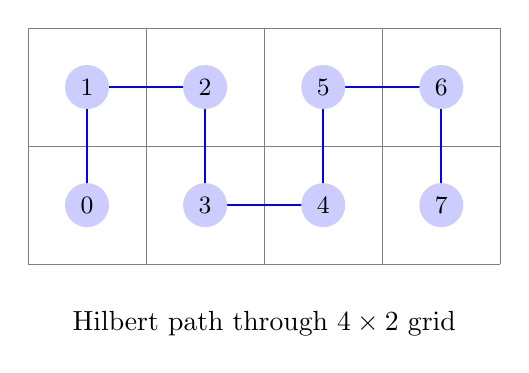
\begin{tikzpicture}[scale=1.5]
    \draw[step=1, gray, very thin] (0,0) grid (4,2);
    % Path: (0,0) -> (0,1) -> (1,1) -> (1,0) -> (2,0) -> (2,1) -> (3,1) -> (3,0)
    \draw[thick, blue, ->]
        (0.5,0.5) -- (0.5,1.5) -- (1.5,1.5) -- (1.5,0.5) --
        (2.5,0.5) -- (2.5,1.5) -- (3.5,1.5) -- (3.5,0.5);
    \foreach \x/\y/\n in {0.5/0.5/0, 0.5/1.5/1, 1.5/1.5/2, 1.5/0.5/3,
                          2.5/0.5/4, 2.5/1.5/5, 3.5/1.5/6, 3.5/0.5/7} {
        \node at (\x,\y) [circle, fill=blue!20, inner sep=3pt] {\small \n};
    }
    \node at (2, -0.5) {Hilbert path through $4 \times 2$ grid};
\end{tikzpicture}
\end{center}

Every step is a unit step: each consecutive pair of indices corresponds to
adjacent points (differing in exactly one coordinate by exactly 1).

% ============================================================================
\section{Summary}
% ============================================================================

\subsection{What We Proved}

\begin{enumerate}
    \item \textbf{Bijection} (Theorem~\ref{thm:bijection}): The \texttt{encode}
          and \texttt{decode} functions are exact inverses. Every point in
          $P(\mathbf{m})$ corresponds to a unique Hilbert index in
          $\{0, \ldots, 2^M - 1\}$, and vice versa.

    \item \textbf{Lattice Continuity} (Theorem~\ref{thm:continuity}):
          Consecutive indices correspond to adjacent lattice points. The
          path visits every point exactly once, taking only unit steps.
\end{enumerate}

\subsection{Key Ideas}

\begin{itemize}
    \item \textbf{Gray codes} ensure that consecutive sub-hypercube indices
          correspond to adjacent sub-hypercubes.
    \item \textbf{The $T$-transform} reorients coordinates while preserving
          adjacency.
    \item \textbf{Activation embedding} correctly handles the transition when
          new axes become active, by treating direction $d$ as a physical
          axis label rather than a positional index.
    \item \textbf{Hierarchical structure}: The proof of continuity uses
          induction on the level where the index digit changes, showing that
          seams between sub-boxes are always unit steps.
\end{itemize}

\subsection{The Bug and the Fix}

Hamilton's original ``compact Hilbert indices'' algorithm has a subtle bug:
it doesn't properly re-index the direction parameter $d$ when axes activate.
This causes incorrect paths at activation boundaries.

The fix---\textbf{activation embedding}---explicitly tracks which physical
axis $d$ refers to and re-indexes it when the active axis set changes. This
maintains the geometric invariant that exit and entry points of adjacent
sub-hypercubes are truly adjacent in the lattice.

% ============================================================================
\appendix
\section{Hamilton's Theorems Referenced}
% ============================================================================

For reference, here are the key results from Hamilton that we use:

\begin{itemize}
    \item \textbf{Theorem 2.1}: $\gc(i) = i \XOR (i \SHR 1)$.
    \item \textbf{Theorem 2.2}: $\bitfn(i, j) = \sum_{k=j}^{m-1} \bitfn(\gc(i), k) \mod 2$.
    \item \textbf{Lemma 2.3}: $\mathrm{g}(i) = \tsb(i)$.
    \item \textbf{Theorem 2.9}: Closed form for $\dir(i)$.
    \item \textbf{Theorem 2.10}: Closed form for $\entry(i)$.
    \item \textbf{Lemma 2.11}: $T_{(e,d)}$ maps entry/exit to $0$/$2^{n-1}$.
    \item \textbf{Lemma 2.12}: Inverse transform formula.
    \item \textbf{Lemma 2.13}: Composed transforms formula.
\end{itemize}

\section{Notation Reference}
% ============================================================================

\begin{center}
\begin{tabular}{cl}
\toprule
Symbol & Meaning \\
\midrule
$n$ & Number of dimensions \\
$m_j$ & Precision (number of bits) for axis $j$ \\
$\mathbf{m}$ & Vector $(m_0, \ldots, m_{n-1})$ \\
$M$ & Total bits: $\sum_j m_j$ \\
$m_{\max}$ & Maximum precision: $\max_j m_j$ \\
$P(\mathbf{m})$ & The dyadic box (set of all lattice points) \\
$s$ & Level index (1 to $m_{\max}$) \\
$k_s$ & Number of active axes at level $s$ \\
$A_s$ & Ordered list of active axes at level $s$ \\
$\ell_s(\mathbf{p})$ & Packed bit-plane word at level $s$ \\
$w_s$ & Index digit for level $s$ \\
$e$ & Entry mask (part of orientation state) \\
$d$ & Direction (part of orientation state) \\
$\XOR$ & Bitwise exclusive-or \\
$\ROTR$ & Bit rotation right \\
$\ROTL$ & Bit rotation left \\
$\gc$ & Gray code function \\
$\gcinv$ & Gray code inverse \\
$T_{(e,d)}$ & The transform: $(b \XOR e) \ROTR (d+1)$ \\
$\entry(i)$ & Entry point of $i$-th sub-hypercube \\
$\exitpt(i)$ & Exit point of $i$-th sub-hypercube \\
$\dir(i)$ & Direction within $i$-th sub-hypercube \\
$\mathrm{g}(i)$ & Axis connecting sub-hypercubes $i$ and $i+1$ \\
\bottomrule
\end{tabular}
\end{center}

\end{document}
